\scanpage{71}

qui est sans doute $=L_i=\operatorname{Ker}(p_i:\mathcal{E}_i\to\Gamma)=$ \unsure{l'}\uline{$\operatorname{Im}$}$(\kappa_i:T(\bar{k})\to\mathcal{E}_i\cap\pi)$.
Donc on trouve que \deleted{\unsure{$f$}} la classe de \deleted{hom.} $\pi$-conjugaison de groupes sur $\Gamma$ de $f:\mathcal{E}'\to\mathcal{E}$ suffit à déterminer le \unsure{hom.} $\mathcal{D}'\to\mathcal{D}$ dans la cat. bordélique.
Je présume qu'un peu de sueur permettrait de prouver que cela marche encore dans le cas général (sans supposer les $\Gamma_i=\operatorname{Im}(\unsure{\mathcal{E}_i}\to\Gamma)$ égaux à $\Gamma$).
Cela signifie (dans le cas actuel) que la structure essentielle qui décrit $(X,S)$ est celle d'\deleted{\illegible{1}} ``\uline{extension extérieure}'' de $\Gamma$ par un groupe $\pi$ [hom. ext. surjectif d'un groupe, de noyau un $\pi$], avec $\pi$ muni d'une \uline{structure à lacets} i.e. \deleted{classe de conjugaison} \inserted{d'hom.} \uline{extérieurs}
\[
\kappa_i:\unsure{T\mu}\,\unsure{(=T\bar{k})}\,\unsure{\overset{\text{non canon}^{t}}{\simeq}}\,\widehat{\mathbf{Z}}\unsure{)}\to\pi
\]
(satisfaisant certaines conditions), les

\margin{70}

\scanpage{72}
\mspage{34}

hom \inserted{de} $\mathcal{E}'\to\Gamma$ (noyau $\pi'$) dans $\mathcal{E}\to\Gamma$ (noyau $\pi$) étant les classes de $\pi$-conjugaison d'homomorphismes $\mathcal{E}'\to\mathcal{E}$ de groupes sur $\Gamma$, induisant des hom $\pi'\to\pi$ compatibles avec la structure à lacets.

9. Structure tangentielle \inserted{``\unsure{intrinsèque|intrinsèques}''} sur les \unsure{S.F.S.|S.E.S.}.
\margin{[Les \unsure{notions} d'extensions ``de deuxième type'']}

\unsure{Revenant|Revenons} à la description de $(X,S)$ par
$\Pi_{D^*}\to\Pi_U\to\Pi_e$, un \unsure{s.f.s.|s.e.s.} correspond donc à une comp. connexe \inserted{$\Pi_{D_i^*}$} de $\Pi_{D^*}$, ou \inserted{un $\Pi_{D_i}$} de son quotient $\Pi_D$ --- considérons
\[
\Pi_{D_i^*}\xrightarrow{\unsure{\sigma_i=\Pi_{f_{D_i^*D_i}}}}\Pi_{D_i}.
\]
On va décrire certaines sections (à isom. près) de ce \deleted{\unsure{fonct}} \inserted{morphisme} de groupoïdes, i.e. des \inserted{couples $(\gamma,\lambda)$} foncteurs
$\Pi_{D_i}\to\Pi_{D_i^*}$ et d'une iso. $\unsure{\sigma_i}\circ\gamma\overset{\lambda}{\simeq}\operatorname{id}$.
Si on choisit un $\widetilde{D}_i^*\in\operatorname{Ob}\Pi_{D_i^*}$ (rev. universel de $D_i^*$) d'où hom \inserted{surj.}
\[
\mathcal{E}_i=\operatorname{Aut}(\widetilde{D}_i^*)\to\Gamma_i
=\operatorname{Aut}(\unsure{\sigma_i}(\widetilde{D}_i^*)=\widetilde{D}_i),
\]
\unsure{la} \deleted{donnée} donnée de $(\gamma,\unsure{\lambda_i|\lambda})$, \inserted{et d'une iso $\gamma(\widetilde{D}_i)\simeq\widetilde{D}_i^*$ donnant l'iso identique par application de $\unsure{\sigma_i}$,} revient à celle d'un hom $\Gamma_i\to\mathcal{E}_i$.
--- et les classes d'isomorphismes des couples $(\gamma,\lambda)$ correspondent aux classes de \inserted{$L_i$}-conjugaison

\margin{71}

\scanpage{73}

($L_i=\operatorname{Ker}(\mathcal{E}_i\to\Gamma_i)$) de \deleted{morphismes} \inserted{sections} de l'ext. $\mathcal{E}_i$ de $\Gamma_i$ par $L_i$.

Ceci posé, \unsure{on a}
\[
\Gamma_i=\operatorname{Gal}(\overline{K}_i/K_i).
\]
où $K_i=k(s_i)$, $\overline{K}_i$ est la clôture algébrique de $K_i$ définie par $\widetilde{D}_i$ (à priori, elle n'est pas \unsure{can\textsuperscript{t}.} isom. à $\overline{K}$ sur $K$\ldots), et les classes de \deleted{\unsure{extensions}} \inserted{scindages} d'extensions forment un \uline{torseur} \inserted{$\Sigma_i$} (s'il y en a, et on sait qu'il y en a\ldots) sous $H^1(\Gamma_i,L_i)$, ou encore, comme $\kappa_i:L_i\xleftarrow{\sim}T(\overline{K}_i)$, sous
\[
H^1(\operatorname{Gal}(\overline{K}_i/K_i),T(\overline{K}_i))
\simeq H^1(K_i,\unsure{T_e|T_\ell}(G_m))
\simeq\varprojlim_n H^1(K_i,\mu_n).
\]
Or la suite exacte de Kummer donne
\diagram{\begin{tikzcd}[ampersand replacement=\&,column sep=small]
0 \arrow[r] \& H^0(K_i,\unsure{G_m})_n \arrow[r] \arrow[d,equal] \& H^1(K_i,\mu_n) \arrow[r] \& {}_nH^1(K_i,G_m) \arrow[r] \arrow[d,equal] \& 0 \\
\& (K_i^*)_n \&\& 0 \&
\end{tikzcd}}
i.e. $H^1(K_i,\mu_n)\simeq(K_i^*)_n$, donc
\[
H^1(K_i,T(G_m))\simeq\varprojlim_n(K_i^*)_n
\]

\margin{72}

\scanpage{74}
\mspage{35}

Notons qu'on a un hom canonique
\[
K_i^*\to\underbrace{H^1(K_i,T(G_m))}_{\mathcal{H}_i}
\simeq\varprojlim(K_i^*{}_n)
\]
dont le noyau est formé des $\unsure{x}\in K_i^*$ tels que pour $\forall\ n\in\mathbf{N}$, on ait $x\in K_i^{*n}$.
Comme $K_i$ est de t.f. sur $\mathbf{Q}$, cet hom est injectif, i.e. $K_i^*$ s'identifie à un sous-groupe de $\mathcal{H}_i$.

Ceci posé, \unsure{on va} définir, dans le torseur $\Sigma_i$ sous $\mathcal{H}_i$ des scindages de $D_i^*$ sur $D_i$, un sous-\inserted{$K_i^*$}-torseur (i.e. un élément de $\Sigma_i/K_i^*$).
Pour ceci,

\deleted{notons que $\mathcal{O}_{s_i}=\widehat{\mathcal{O}}_{X,s_i}$ contient canoniquement le sous-corps $K_i$ (p.ex. comme clôture entière de $K$ dans $\mathcal{O}_{s_i}$), et que le choix d'une uniformisante $t$ de $\mathcal{O}_{s_i}$ définit un \deleted{sous-corps \illegible{1}} \inserted{$K_i$-}isom $\mathcal{O}_{s_i}\simeq K_i[[T]]$, (par la condition $T\mapsto t$). Notons que l'on a}

\margin{73}

\scanpage{75}

\deleted{(avec $\widetilde{D}_i^*$) une clôture algébrique \inserted{$\overline{K}_s$} de $K_s$ (corps des fractions de $\mathcal{O}_s$), définissant \deleted{\illegible{2}} \inserted{une} clôture alg. $\unsure{\overline{K}_i}$ de $K_i=k(s_i)$, \unsure{qui n'est autre} justement que $\overline{K}_i$. \deleted{Ceci posé, dans $\overline{K}_s$ le sous-corps}}
\margin{faire un raisonnement local général, en laissant tomber l'indice $i$.}

Considérons plus généralement le cas d'un corps $\unsure{k|h}$ $(=K_i)$ de car. $0$, et d'une \deleted{\illegible{1}} $\unsure{k|h}$-algèbre $\mathcal{O}$ qui est \inserted{\unsure{jauge}} hensélienne de corps résiduel $\unsure{k|h}$.
\inserted{soit $\unsure{L|K}$ le corps des fractions de $\mathcal{O}$}
On va, pour \unsure{t\textsuperscript{te}} uniformisante $t$ de $\mathcal{O}$, définir une section $(\gamma,\lambda)$ \unsure{du|des} \deleted{\unsure{la caté}} \unsure{groupoïde|groupoïdes} des clôtures alg. de $\unsure{L|K}$, vers celui des rev. universels de $\unsure{\operatorname{f\acute{e}t}(\mathcal{O})|\operatorname{fin}(\mathcal{O})}$ ou, ce qui revient au même, des clôtures alg. de $\unsure{k|h}$. Pour ceci,

soit
\[
\mathcal{O}(n,\unsure{t|s})=\mathcal{O}[T_n]/(T_n^n-s),\quad\text{et}
\]
\[
\mathcal{O}(\infty,t)=\varinjlim_n\mathcal{O}(n,t),\quad
\text{par }\unsure{\overline{T}_n\mapsto\overline{T}_{mn}^{\,m}}.
\]
\deleted{alors $\mathcal{O}(\infty,t)$ est \unsure{encore une} jauge hensélienne}
\deleted{\illegible{1}}
$\unsure{L|K}(n,t)=\mathcal{O}(n,t)\otimes_{\mathcal{O}}K=$ corps des fractions de $\mathcal{O}(n,t)$, $\unsure{L|K}(\infty,t)=\varinjlim_n\unsure{L|K}(n,t)$ le corps des fractions de $\mathcal{O}(\infty,t)$. C'est

\margin{74}

\scanpage{76}
\mspage{36}

une ext. alg. de $\unsure{L|K}$, et pour \unsure{t\textsuperscript{te}} \deleted{clôture alg. $\overline{k}$ de $k$, \illegible{1} $L\otimes_k\overline{k}$ est alg. clos} \inserted{extension finie, ou ind-finie} $k'$ de $k$, posons $\mathcal{O}'=\mathcal{O}\otimes_k k'$ (qui est aussi une jauge hensélienne sur $k'$ de corps résiduel $k'$, de corps des fractions $L'\simeq\unsure{L|K}\otimes_k k'$), on a \inserted{des iso can.} \deleted{\illegible{1}}
\[
\mathcal{O}(\unsure{n|\infty},t)\otimes_{\mathcal{O}}\mathcal{O}'\simeq\mathcal{O}'(\unsure{n|\infty},t)
\]
\[
\mathcal{O}(\infty,t)\otimes_{\mathcal{O}}\mathcal{O}'\simeq\mathcal{O}'(\infty,t)
\]
d'où
\[
\unsure{L|K}(\unsure{n|\infty},t)\otimes_k\unsure{\overline{k}'|k'}\simeq\unsure{L'|K'}(\unsure{n|\infty},t)
\]
\[
L(\infty,t)\otimes_k k'\simeq L'(\infty,t)
\]
Or si $\unsure{k'|\overline{k}'}$ est alg clos, \deleted{on sait que} $\mathcal{O}'$ str. hensélien, on sait que $L'(\infty,t)$ est \unsure{alors} alg. clos.
\deleted{\unsure{D'autre part} \illegible{1}} comme $\unsure{\overline{k}'|k'}\subset\mathcal{O}'(\infty,t)\subset L'(\infty,t)$, dans ce cas $k'$ \deleted{\illegible{1}} s'identifie à la clôture alg. \inserted{$\overline{k}$} de $k$ dans $L'(\infty,t)=\overline{L}$.
Donc on a bien trouvé une section de $\Pi_{D^*}$ sur $\Pi_D$.

Mais si on remplace $s$ par $s'=su^n$, avec $u\in\mathcal{O}^*$, on trouve des iso
\diagram{$\unsure{\lambda(n,u)}:\quad$\begin{tikzcd}[ampersand replacement=\&,column sep=large]
\mathcal{O}(n,s) \arrow[r] \arrow[d,equal] \& \mathcal{O}(n,s') \arrow[d,equal] \\
\mathcal{O}[T_n]/(T_n^n-s) \& \mathcal{O}[T_n]/(T_n^n-s')
\end{tikzcd}}
par $\overline{T}_n\to u\overline{T}_n$
d'où par passage à la limite
\[
\lambda(\infty,u):\mathcal{O}(\infty,s)\unsure{\longrightarrow}\mathcal{O}(\infty,s')
\]
induisant $L(\infty,s)\xrightarrow{\sim}L(\infty,s')$ isom d'ext.

\margin{75}

\scanpage{77}

d'où un isom entre les sections correspondantes de $\Pi_{\unsure{D^*|L}}$ sur $\Pi_k$.
Ceci implique que si $s,s'$ diffèrent par un $u\in\mathcal{O}^*$ tel que son image dans $k$ soit $1$ \deleted{(donc $u\in$ \illegible{2}} \inserted{i.e. $u\in1+m$} (qui est un s.-groupe divisible de $\mathcal{O}^*$\unsure{]|)}) alors $s,s'$ définissent des sections isomorphes.
On trouve donc une application canonique
\[
\begin{array}{ccl}
(m/m^2)^* & \to &
\begin{gathered}
\text{classes d'iso de sections de}\\
\Pi_L\text{ sur }\Pi_k\quad\text{i.e. de}\\
\operatorname{Gal}(\overline{L}/L)\to\operatorname{Gal}(\overline{k}/k)
\end{gathered}
\\[1ex]
\begin{gathered}
\deleted{\unsure{\text{(et}}}\text{(ens des}\\
\text{bases de }m/m^2\text{)}\\
\text{qui est un}\\
\text{torseur sous}\\ k^*
\end{gathered}
&&
\begin{gathered}
\text{(qui est un torseur sous}\\
H^1(\operatorname{Gal}(\overline{k}/k),T(\overline{k}))\\
\text{ou sous }H^1(k,T(G_m))\ldots)
\end{gathered}
\end{array}
\]

On constate aussitôt que cette application est compatible avec l'hom
\[
\Theta:k^*\to H^1(k,T(G_m))
\]
sur les groupes d'op. de ces torseurs.
Dans le cas où cet hom est injectif (p.ex. $k$ \deleted{\illegible{6}} de t.f. sur $\mathbf{Q}$) on trouve donc un plongement de $\unsure{m/m^2}$ comme un sous $\Theta[k^*]$-torseur du $H^1(k,T(G_m))$-torseur

\margin{76}

\scanpage{78}
\mspage{37}

des scindages de $\Pi_{D^*}$ \inserted{($\simeq$ groupoïde des clôtures alg. de $L$)} sur $\Pi_D$ ($\simeq$ groupoïde des clôtures alg. de $\unsure{k}$).

Revenant au cas des \deleted{\illegible{1}} $\Pi_{D^*}\to\Pi_U\to\Pi_e$ $\unsure{\kappa|K}\ldots$, et des \deleted{\illegible{1}}
\[
\mathcal{D}:T(\overline{k}^*)\xrightarrow{\kappa_i}\mathcal{E}_i\hookrightarrow\mathcal{E}\xrightarrow{p}\Gamma
\]
qui les explicitent, on trouve donc une structure supplémentaire sur $\mathcal{E}$ ou $\mathcal{D}$ via \deleted{\unsure{sur}} les Ext. $\mathcal{E}_i$ de $\Gamma_i\subset\Gamma$ par $T(\overline{k}^*)$, à savoir \deleted{\unsure{des}} \inserted{$\forall i\in I$} sous-$K_i^*$-torseurs dans le torseur sous
$H^1(K_i,\unsure{\Pi|T}(G_m))\simeq\varprojlim\unsure{(K_i^*)_n}$ des \inserted{classes de} scindages de $\mathcal{E}_i$.
Il faudrait expliciter le comportement de cette structure suppl. relativement à des morphismes (provenant de situations géométriques) et la relation avec la norme des $1$-formes différentielles --- j'ai la flemme de l'expliciter en long et en large !

La chose essentielle que je retiens surtout, c'est que pour $I\ne\varnothing$ et les $\mathcal{E}_i\to\Gamma$ surjectifs (pour simplifier), on trouve \inserted{$\forall i$} \unsure{des|une} ``\unsure{familles|famille} \unsure{transcendantes|transcendante}'' de scindages de $\mathcal{E}\to\Gamma$ (via scindages de $\mathcal{E}_i$ sur $\Gamma$) --- \unsure{ess.\textsuperscript{t}} \unsure{indexées}

\margin{77}

\scanpage{79}

par $H^1(\unsure{K_i|K},T(G_m))\simeq\varprojlim(K^*)_n$ (plus précisément, par un torseur sous ledit)

--- dans cette famille, une sous-famille de scindages qu'on peut qualifier de ``géométriques'', indexée par $K^*$ (plus précisément, un sous-torseur\ldots).
On vérifie que les \inserted{classes de $\pi$-}scindages obtenus pour des indices $i,i'$ distincts sont distinctes, même en se ramenant aux \unsure{$\pi$-}scindages corr. de l'ext. de $\Gamma$ par $\pi_{\mathrm{ab}}$ déduite de l'ext. $\mathcal{E}$ de $\Gamma$ par $\pi$ (je ne fais pas le détail des vérifications, via Mordell-Weil\ldots) et distincts des scindages associés aux pts. rat$/K$ de $X\backslash S$.

\margin{\figure{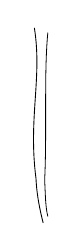
\begin{tikzpicture}[x=1cm,y=1cm,line cap=round]
\draw[line width=.32pt] (0,0) .. controls (.10,-.64) and (-.08,-1.14) .. (.02,-1.91)
 .. controls (.03,-2.14) and (.08,-2.35) .. (.11,-2.47);
\draw[line width=.29pt] (.17,-.06) .. controls (.12,-.59) and (.16,-1.31) .. (.13,-1.93)
 .. controls (.14,-2.13) and (.14,-2.27) .. (.17,-2.39);
\end{tikzpicture}}}
Il faudrait envisager la conj. bordélique dans le cas (\uline{\unsure{III|IV}}), en énonçant (sous toutes réserves, encore !) qu'il n'y a (peut-être) pas d'autres scindages de l'ext. $\mathcal{E}$ de $\Gamma$ par $\pi$ que ceux-ci ....

\margin{78}

\scanpage{80}
\mspage{38}

10. Ajustement des hypothèses (\unsure{remords|remarques}).

Je me rends compte que dans la définition des morphismes $(X',S')\xrightarrow{f}(X,S)$, l'hypothèse $f^{-1}(S)_{\mathrm{red}}=S'$ est étriquée --- il faut prendre des morphismes \uline{quelconques} $f:X'\backslash S'\to X\backslash S$ (se prolongeant bien sûr en $\widehat{f}:X'\to X$).
On aura donc $S'\supset\widehat{f}^{-1}(S)_{\mathrm{red}}$, mais $S'$ peut être strictement plus grand que $\widehat{f}^{-1}(S)_{\mathrm{red}}$.
Il faut donc ajuster en conséquence la description de la ``catégorie bordélique'' --- les objets restent des diagrammes de groupoïdes
\[
\mathcal{D}:\Pi_{D^*}\to\Pi_U\to\Pi_e
\]
(plus donnée de \unsure{Kummer}) mais un morphisme $f$ d'un $\mathcal{D}'$ dans un $\mathcal{D}$ ne définit plus nécessairement un $\Pi'_{D^*}\to\Pi_{D^*}$ (en plus de $\Pi'_U\to\Pi_U$) il faut se donner une partie $I'_f$ de $I'=\pi_0(\Pi'_{D^*})$, et se donner seulement
\[
\Pi'_{D^*,I'_f}\xrightarrow{f_{D^*}}\Pi_{D^*}
\]
(avec donnée de commutation \inserted{$\unsure{\alpha_{D^*U}}$} relatif au carré avec $f_U$).
Bien sûr, dans la description en termes de $\mathcal{E}',\mathcal{E}$ etc., on exige que pour $i'\in I'\backslash I'_f$, $f_{\mathcal{E}}:\mathcal{E}'\to\mathcal{E}$ est trivial sur $\unsure{\mathcal{E}'_{i'}|\xi'_{i'}}\subset\mathcal{E}'$ --- et \unsure{reste|c'est} défini comme $I'_f\to I$ ; les données relatives aux $i'\in$

\margin{79}
